  \documentclass[9pt, aspectratio=169]{beamer}

  \usetheme{metropolis}
  \setbeamertemplate{itemize items}{\faAngleRight}

  \metroset{titleformat=smallcaps,block=fill,numbering=counter,progressbar=frametitle,sectionpage=none}
\setbeamersize{text margin left=5mm,text margin right=5mm} 
% \input{embed_video}
\usepackage{fontspec,minted}
\usepackage[scale=1]{ccicons}
\usepackage{metalogo}
\usepackage{xcolor,colortbl}
\usepackage{multicol,multirow,booktabs}
\usepackage{appendixnumberbeamer}
\usepackage{graphicx}
\usepackage{mismath}
\usepackage{bm}
\usepackage{fontawesome5}
\usepackage{csquotes}
\usepackage[backend=biber, natbib, sorting=nyt, doi=true, url=false, url=false, isbn=false, maxbibnames=10]{biblatex}
\addbibresource{../utils/refs.bib}

\usepackage[spanish, es-nodecimaldot]{babel}
\deftranslation[to=spanish]{Definition}{Definición}
\deftranslation[to=spanish]{Theorem}{Teorema}
\deftranslation[to=spanish]{Example}{Ejemplo}

\usepackage{mathtools, mathrsfs}
\usefonttheme{professionalfonts}
\usepackage{textcomp, wasysym}

\setsansfont[BoldFont={Iwona Heavy}, Numbers={Lining, Proportional}]{Iwona Light}
\setmonofont[Scale=MatchLowercase]{Hack Nerd Font Mono}

\setbeamercolor{alerted text}{fg=red,bg=black!2}
\setbeamercolor{progress bar}{fg=red,bg=red!2}
\setbeamertemplate{itemize item}{\faCaretRight}
\setbeamertemplate{itemize subitem}{ \faAngleRight}
\setbeamertemplate{blocks}[shadow=false]
\setbeamercolor{block title}{bg=black!30,fg=red}
\setbeamercolor{block body}{bg=black!20,fg=black}
\setbeamertemplate{theorem begin}
{%
\begin{\inserttheoremblockenv}
{%
\inserttheoremheadfont
%{Teorema:}
\inserttheoremname
\ifx\inserttheoremaddition\@empty\else\ : \inserttheoremaddition\fi%
\inserttheorempunctuation
}%
}
\setbeamertemplate{theorem end}{\end{\inserttheoremblockenv}}
\makeatother


 
\usepackage{gensymb,amssymb}
\usepackage{siunitx}
\DeclareSIUnit{\nada}{\relax}
\usepackage{upquote}
\usepackage{cancel}
\usepackage{algpseudocode}
\algrenewcommand\algorithmicrequire{\textbf{Requiere}}
\algrenewcommand\algorithmicensure{\textbf{Devuelve}}
\setbeamertemplate{blocks}[shadow=false]

\newcommand{\cx}{\column{0.5\textwidth}}
\newcommand{\cw}[1]{\column{#1\textwidth}}

\author{Manuel Carlevaro}
\date{{\tiny Departamento de Ingeniería Mecánica \\
             Grupo de Materiales Granulares - UTN FRLP \\
             manuel.carlevaro@gmail.com }}
\institute{
  \vspace{6em}
  \centering
  {\tiny
  Cálculo Avanzado \enspace • \enspace 2025 \\
    \faLinux \- $\cdot$ \- \fontspec{TeX Gyre Pagella}\XeLaTeX \- $\cdot$ \- \ccbysa }
}

%% Operadores
\DeclareMathOperator{\sen}{sen}
\DeclareMathOperator{\senc}{senc}
\DeclareMathOperator{\sign}{sign}
\DeclareMathOperator{\Tr}{Tr}
\DeclareMathOperator{\rg}{rg}
\DeclareMathOperator{\cond}{cond}
\newcommand{\T}[1]{\underline{\bm{#1}}}
\newcommand{\uvec}[1]{\hat{\bm{#1}}}

\usepackage{hyperref}
\hypersetup{
    colorlinks,
    citecolor=blue,
    filecolor=black,
    linkcolor=blue,
    urlcolor=blue
}
\urlstyle{same}

%% Códigos
\usepackage{minted}
\newminted[cpp]{cpp}{linenos,fontsize=\footnotesize,frame=lines,numbersep=4pt}
\newmintedfile[cppcode]{cpp}{linenos,fontsize=\footnotesize,frame=lines,numbersep=4pt}
\newcommand{\mic}[1]{\mintinline{C++}{#1}}

\newminted[py]{python}{linenos,fontsize=\footnotesize,frame=lines,numbersep=4pt}
\newminted[pyc]{pycon}{linenos,fontsize=\footnotesize,frame=lines,numbersep=4pt} % Consola de Python
\newminted[ipy3]{ipython3}{linenos,fontsize=\footnotesize,frame=lines,numbersep=4pt} % Consola de iPython3
\newmintedfile[pycode]{python}{linenos,fontsize=\footnotesize,frame=lines,numbersep=4pt}

\newmintedfile[makef]{basemake}{linenos,fontsize=\footnotesize,frame=lines,numbersep=4pt}
\definecolor{bg}{RGB}{22,43,58}
\newminted[shell]{console}{linenos=false,fontsize=\footnotesize,breaklines=true, frame=single} % Linea de comandos
\renewcommand\listingscaption{Código}

\makeatletter
\AtBeginEnvironment{minted}{\dontdofcolorbox}
\def\dontdofcolorbox{\renewcommand\fcolorbox[4][]{##4}}
\makeatother

% uso:
% Ejemplo de uso explícito:
% \begin{py}
% >>> list("abcd")
% ['a', 'b', 'c', 'd']
% \end{py}
% 
% Ahora ejemplo de código en file:
% \pycode{Chapters/intro/code/hola.py}
% 
% También se puede poner un sector del file:
% \pycode[firstline=6, lastline=7]{Chapters/intro/code/hola.py}
% 
% También se puede poner código \textit{inline}: \mip{print('¡Hola mundo!')} y en una sola línea:
% \slp|if __name__ == '__main__')|
% 
% Por último, se puede poner el código en un entorno \textit{float}, esto es, como las tablas y las figuras, con un caption y un label para luego hacer referencias, como por ejemplo al Código \ref{code:hola}.


\usepackage{tikz}
\usetikzlibrary{shapes,shadows,arrows,positioning,matrix,chains,backgrounds,fit}

\tikzset{
    %Define standard arrow tip
    >=stealth',
    %Define style for boxes
    obj/.style={
           rectangle,
           rounded corners,
           draw, very thick,
           text width=10em, fill=green!20,
           minimum height=2em,
           text centered, drop shadow},
    proc/.style={
	    rectangle, rounded corners,
	    draw,fill=red!50,very thick,
	    text width=8em,minimum height=2em,
	    text centered, drop shadow},
    % Define arrow style
    pil/.style={
           ->,
           thick,
           shorten <=2pt,
           shorten >=2pt,}
}

\setbeamertemplate{bibliography item}{%
  \ifboolexpr{ test {\ifentrytype{book}} or test {\ifentrytype{mvbook}}
    or test {\ifentrytype{collection}} or test {\ifentrytype{mvcollection}}
    or test {\ifentrytype{reference}} or test {\ifentrytype{mvreference}} }
    {\setbeamertemplate{bibliography item}{\faBook}}
    {\ifentrytype{online}
            {\setbeamertemplate{bibliography item}{\faGlobe}}
   {\setbeamertemplate{bibliography item}{\faFileText}}}%
  \usebeamertemplate{bibliography item}}

\defbibenvironment{bibliography}
  {\list{}
     {\settowidth{\labelwidth}{\usebeamertemplate{bibliography item}}%
      \setlength{\leftmargin}{\labelwidth}%
      \setlength{\labelsep}{\biblabelsep}%
      \addtolength{\leftmargin}{\labelsep}%
      \setlength{\itemsep}{\bibitemsep}%
      \setlength{\parsep}{\bibparsep}}}
  {\endlist}
  {\item}
\newcommand{\bcite}[1]{\citeauthor{#1}, \citetitle{#1} (\citeyear{#1})}


  \title{Normas de vectores y matrices}
  \subtitle{}

  %%%%
  % Bibliografía
  % Brian Bradie - A Friendly Introduction to Numerical Analysis - Section 3.3 pg 185
  % Alfio Quarteroni et al - Numerical Mathematics - Sec. 1.10 pg 36
  %%%%

  \begin{document}
  \maketitle

  \section{Introducción}

  \begin{frame}
  \begin{columns}[t]
  \cx
  \textbf{Motivación:}

  Error en escalar:
  \[ |x^* - x| \sim \delta x \]

  ¿Cómo es el error en $\mathbb{R}^n$ o en $\mathbb{R}^{m \times n}$?

  \[ \bm{x} \mapsto \delta \bm{x} \]
  o
  \[ (\bm{A} + \delta \bm{A})(\bm{x} + \delta \bm{x}) = \bm{b} + \delta \bm{b} \]
  \pause

  \begin{definition}[Espacio vectorial]
  Un \textit{espacio vectorial} sobre el cuerpo $K$ ($K = \mathbb{R}$ o $K = \mathbb{C}$), es un conjunto no vacío $V$, cuyos elementos se denominan \textbf{vectores}, y en el que se definen dos operaciones: \textbf{suma} y \textbf{multiplicación escalar}.
  \end{definition} \pause

  \cx
  \textbf{Propiedades:}
  \begin{enumerate}
      \item La suma es conmutativa y asociativa.
      \item $\exists\; \bm{0} \in V$ (vector cero o nulo) tal que $\bm{v} + \bm{0} = \bm{v}, \; \forall \bm{v} \in V$.
      \item $0 \cdot \bm{v} = \bm{0}, 1 \cdot \bm{v} = \bm{v}$, donde $0$ y $1$ son respectivamente el cero y uno de $K$.
      \item $\forall \bm{v} \in V, \exists -\bm{v} \in V : \bm{v} + (-\bm{v}) = \bm{0}$.
      \item Propiedad distributiva:
          \begin{itemize}
          \item $\forall \alpha \in K, \forall \bm{v}, \bm{w} \in V, \alpha(\bm{v} + \bm{w}) = \alpha \bm{v} + \alpha \bm{w}$.
          \item $\forall \alpha, \beta \in K, \forall \bm{v} \in V, (\alpha + \beta) \bm{v} = \alpha \bm{v} + \beta \bm{v}$.
          \end{itemize}
      \item Propiedad asociativa:
          \begin{itemize}
              \item $\forall \alpha, \beta \in K, \forall \bm{v} \in V, (\alpha \beta)\bm{v} = \alpha (\beta \bm{v})$
          \end{itemize}
  \end{enumerate} \pause

  \textbf{Ejemplos:}
  \begin{itemize}
      \item $V = \mathbb{R}^n \, (V = \mathbb{C}^n), \; n > 1$.
      \item $V = \mathbb{P}_n = \{ p_n(x) = \sum_{k=0}^n a_k x^k \}, \; n \geq 0$.
      \item $V = \mathcal{C}^p([a, b]), \; 0 \leq p \leq \infty$.
  \end{itemize}
  \end{columns}
  \end{frame}

\begin{frame}
\begin{columns}[t]
\cx
\begin{definition}[Producto escalar]
  Un \textbf{producto escalar} en $V$ definido sobre $K$ es cualquier mapeo $\langle \cdot, \cdot \rangle$, $V \times V \mapsto K$ con las siguientes propiedades:
\begin{enumerate}
  \item Es lineal respecto de los vectores en $V$:
      \[ \langle \gamma \bm{x} + \lambda \bm{z}, \bm{y} \rangle = \gamma \langle \bm{x}, \bm{y} \rangle + \lambda \langle \bm{z}, \bm{y} \rangle \]
      $\forall \bm{x}, \bm{y}, \bm{z} \in V, \; \forall \gamma, \lambda \in K$.
  \item Es hermítico:
      \[ \langle \bm{y},\bm{x} \rangle = \overline{ \langle \bm{x}, \bm{y} \rangle }, \, \forall \bm{x}, \bm{y} \in V \]
  \item Es definido positivo:
      \[ \langle \bm{x}, \bm{x} \rangle \geq 0, \quad \langle \bm{x}, \bm{x} \rangle = 0 \Leftrightarrow \bm{x} = \bm{0} \]
\end{enumerate}
\end{definition} \pause


\cx
\begin{definition}[Norma vectorial]
  Sea $V$ un espacio vectorial sobre $K$. El mapeo $\lVert \cdot \rVert \mapsto \mathbb{R}$ es una \textbf{norma} si se cumple que:
  \begin{enumerate}
      \item (i) $\lVert \bm{v} \rVert \geq 0 \; \forall \bm{v} \in V$ y (ii) $\lVert \bm{v} \rVert = 0 \Leftrightarrow \bm{v} = \bm{0}$;
      \item $\lVert \alpha \bm{v} \rVert = |\alpha| \lVert \bm{v} \rVert \; \forall \alpha \in K , \, \forall \bm{v} \in V$ (propiedad de homogeneidad);
      \item $\lVert \bm{v} + \bm{w} \rVert \leq \lVert \bm{v} \rVert + \lVert \bm{w} \rVert \; \forall \bm{v}, \bm{w} \in V$ (desigualdad triangular),
  \end{enumerate}
  donde $|\alpha|$ denota el valor absoluto de $\alpha$ si $K = \mathbb{R}$, o el módulo de $\alpha$ si $K = \mathbb{C}$. El par $(V, \lVert \cdot \rVert)$ se denomina \textbf{espacio normado}.
\end{definition}
\end{columns}
\end{frame}

\begin{frame}
\begin{columns}[t]
\cx
  \textbf{Ejemplo:} Norma $p$, o $l_p$,  $(\mathbb{R}^n, \lVert \cdot \rVert_p)$
  \[ \lVert \bm{x} \rVert = \left(\sum_{i = 1}^n |x_i|^p\right)^{1/p}, \quad 1 \leq p \leq \infty \]
  \begin{itemize}
      \item Cuando $p \rightarrow \infty$ ($l_{\infty}$): \textbf{norma infinita} o \textbf{norma máxima}
          \[ \lVert \bm{x} \rVert_{\infty} = \max_{1 \leq i \leq n} |x_i| \]
      \item Cuando $p = 1$ ($l_1$): \textbf{norma del taxista}
          \[ \lVert \bm{x} \rVert_1 = \sum_{i = 1}^n |x_i| \]
      \item Cuando $p = 2$ ($l_2$): \textbf{norma euclídea}
          \[ \lVert \bm{x} \rVert_2 = \langle \bm{x}, \bm{x} \rangle^{1/2} = \left(\sum_{i = 1}^n |x_i|^2\right)^{1/2} \]
\end{itemize} \pause

\cx
\textbf{Interpretación gráfica en $\mathbb{R}^2$}:
\begin{columns}
\cx
\begin{center}
  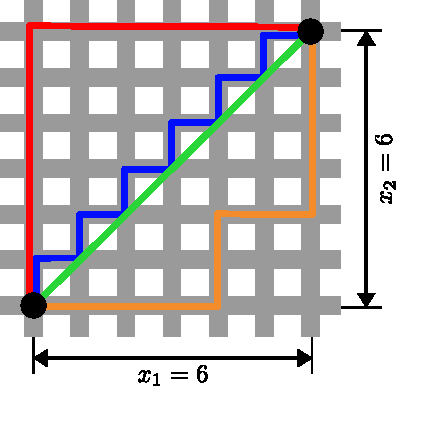
\includegraphics[scale=0.55]{figs/normas-01.pdf}
\end{center}
\cx
\begin{align*}
  \bm{x} &= [6, 5] \\
  l_{\infty} &= \max \{|6|, |5| \} = 6
\end{align*}
Camino más corto:
\begin{itemize}
  \item  $l_1 \; {\color{red} \blacksquare }, {\color{blue} \blacksquare }, {\color{orange} \blacksquare }$: $11$
  \item $l_2 \; {\color{green} \blacksquare}$ : $\sqrt{61} \approx 7.81$
\end{itemize}
\end{columns} \pause

\textbf{Desigualdad de Cauchy-Schwarz:} $\forall \bm{x}, \bm{y} \in \mathbb{R}^n$:
\[ | \langle \bm{x}, \bm{y} \rangle | \leq \lVert \bm{x}  \rVert_2 \lVert \bm{y} \rVert_2 \]
donde la igualdad vale si y solo si $\bm{y} = \alpha \bm{x}, \alpha \in \mathbb{R}$.

\textbf{Continuidad:} Cualquier $\lVert \cdot \rVert$ en $V$ es una \textbf{función continua} de sus argumentos: $\forall \varepsilon > 0, \exists C > 0$ tal que si $\lVert \bm{x} - \hat{\bm{x}} \rVert \leq \varepsilon$, entonces $| \lVert \bm{x} \rVert - \lVert \hat{\bm{x}} \rVert | \leq C \varepsilon$ para cualquier $\bm{x}, \hat{\bm{x}} \in V$.
\end{columns}
\end{frame}

\begin{frame}
\begin{columns}[t]
\cw{0.45}
\textbf{Cálculo de normas:}
\begin{align*}
  \bm{x}_1 &= [1, -2, 3] \\
  \bm{x}_2 &= [2, 0, -1, 2] \\
  \bm{x}_3 &= [0, 1, -4, 2, -1] \\
\end{align*}

\textbf{Norma máxima:}
\begin{align*}
\lVert  \bm{x}_1 \rVert_{\infty} &= \max \{|1|, |-2|, |3|\} = 3\\
\lVert  \bm{x}_2 \rVert_{\infty} &= \max \{|2|, |0|, |-1|, |2|\} = 2\\
\lVert  \bm{x}_3 \rVert_{\infty} &= \max \{|0|, |1|, |-4|, |2|, |-1|\} = 4 \\
\end{align*}

\cw{0.55}
\textbf{Norma $l_1$:}
\begin{align*}
\lVert  \bm{x}_1 \rVert_1 &=  |1| + |-2| + |3| = 6\\
\lVert  \bm{x}_2 \rVert_1 &= |2| + |0| + |-1| + |2|= 5\\
\lVert  \bm{x}_3 \rVert_1 &= |0| +|1| + |-4| + |2| + |-1| = 8 \\
\end{align*}

\textbf{Norma $l_2$:}
\begin{align*}
  \lVert  \bm{x}_1 \rVert_2 &= \sqrt{|1|^2 + |-2|^2 + |3|^2} = \sqrt{14} \approx 3.74\\
  \lVert  \bm{x}_2 \rVert_2 &= \sqrt{|2|^2 + |0|^2 + |-1|^2 + |2|^2}= \sqrt{9} =3\\
  \lVert  \bm{x}_3 \rVert_2 &= \sqrt{|0|^2 +|1|^2 + |-4|^2 + |2|^2 + |-1|^2} = \sqrt{22} \approx 4.69\\
\end{align*}
\end{columns}
\end{frame}

\begin{frame}
%% Ver Burden Faires 9th Edition (Inglés) pg 438
\begin{columns}[t]
\cx
\begin{definition}[Norma matricial]
  Una \textbf{norma matricial} es un mapeo $\lVert \cdot \rVert : K^{m \times n} \rightarrow \mathbb{R}$ tal que:
\begin{enumerate}
  \item $\lVert \bm{A} \rVert \geq 0 \; \forall \bm{A} \in K^{m \times n}$ y $\lVert \bm{A} \rVert = 0 \Leftrightarrow \bm{A} = \bm{0}$;
  \item $\lVert \alpha \bm{A} \rVert = |\alpha| \lVert \bm{A} \rVert, \; \forall \alpha \in K, \forall \bm{A} \in K^{m \times n}$ (homogeneidad);
  \item $\lVert \bm{A} + \bm{B} \rVert \leq \lVert \bm{A} \rVert + \lVert \bm{B} \rVert, \, \forall \bm{A}, \bm{B} \in K^{m \times n}$ (desigualdad triangular).
\end{enumerate}
\end{definition}

La \textbf{distancia entre matrices $m \times n$} con esta norma es $\lVert \bm{A} - \bm{B} \rVert$.
\pause

\cx

\textbf{Norma por componentes:}

Matriz $m \times n \mapsto$ vector $m \cdot n$. Sea $\bm{A} = [a_{ij}] \in \mathbb{C}^{m \times n}$:
\begin{itemize}
  \item \textbf{Norma $p$:}
      \[ \lVert \bm{A} \rVert_p = \left( \sum_{i=1}^m \sum_{j=1}^n |a_{ij}|^p \right)^{1/p} \]
  \item \textbf{Norma de Frobenius:} ($p = 2$)
\[ \lVert \bm{A} \rVert_F^2 = \sum_{i=1}^m \sum_{j=1}^n |a_{ij}|^2 \]
\item \textbf{Norma máxima:}
  \[ \lVert \bm{A} \rVert_{\text{máx}} = \max_{\substack{1 \leq i \leq m \\ 1 \leq j \leq n}} |a_{ij}| \]
\end{itemize}

\end{columns}
\end{frame}

\begin{frame}
\begin{columns}[t]
\cx
\begin{theorem}[Norma inducida]
  Si $\norm{\cdot}$ es una norma vectorial en $K^n$, entonces
  \[ \norm{\bm{A}} = \max_{\norm{\bm{x}} = 1} \norm{\bm{A} \bm{x}} \]
es la norma matricial \textbf{natural} o \textbf{inducida} asociada con la norma vectorial.
\end{theorem}
Alternativamente: 
\[ \norm{\bm{A}} = \max_{\bm{z} \neq \bm{0}} \frac{ \norm{\bm{A} \bm{z}}}{\norm{\bm{z}}} \]

\textbf{Corolario:} $\forall \bm{z} \neq \bm{0}, \bm{A}$ y cualquier norma natural $\norm{\cdot}$:
\[ \norm{\bm{A} \bm{z}} \leq \norm{\bm{A}} \cdot \norm{\bm{z}} \]
\pause

\cx
\textbf{Interpretación gráfica en $\mathbb{R}^2$:}
\begin{center}
  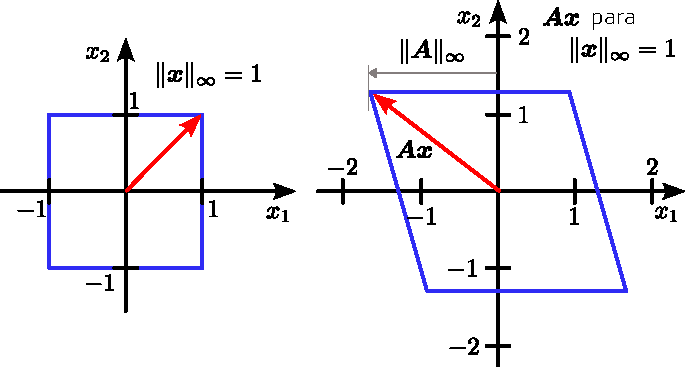
\includegraphics[scale=0.6]{figs/nmat-01.pdf}
\end{center}
\begin{center}
  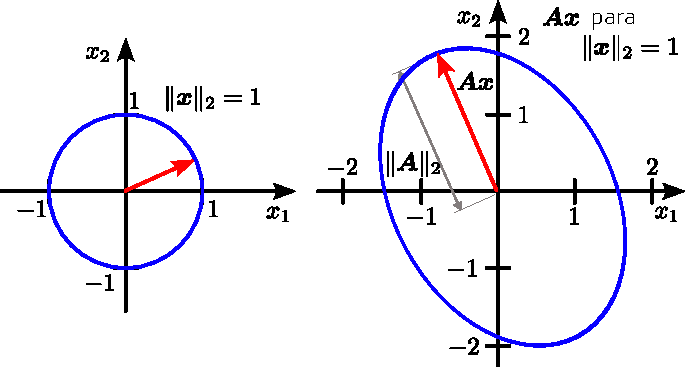
\includegraphics[scale=0.6]{figs/nmat-02.pdf}
\end{center}
\end{columns}
\end{frame}

\begin{frame}
\begin{columns}[t]
\cx
\textbf{Norma inducida $l_p$:} si $\bm{A}$ es una matriz en $K^{m \times n}$
\[ \lVert \bm{A} \rVert_p = \max_{\bm{x} \neq \bm{0}} \frac{ \lVert \bm{A} \bm{x}\rVert_p }{\lVert \bm{x} \rVert_p} \]
\begin{itemize}
  \item \textbf{Norma inducida $l_1$:} (norma suma columna)
      \[ \norm{\bm{A}}_1 = \max_{1 \leq j \leq n} \sum_{i=1}^m |a_{ij}| \]
  \item \textbf{Norma inducida ${\infty}$:} (norma suma fila)
      \[ \norm{\bm{A}}_{\infty} = \max_{1 \leq i \leq m} \sum_{j=1}^n |a_{ij}| \]
  \item \textbf{Norma inducida $l_2$:} $\mapsto$ \alert{próxima clase}.
\end{itemize}
\pause

\cx
\begin{definition}[Norma sub-multiplicativa]
  Una norma matricial $\lVert \cdot \rVert$ es \textbf{sub-multiplicativa} si $\forall \bm{A} \in K^{n \times m}, \forall \bm{B} \in K^{m \times q}$:
  \[ \lVert \bm{A} \bm{B} \rVert \leq \lVert \bm{A} \rVert \lVert \bm{B} \rVert \]
\end{definition}

\begin{definition}[Consistencia]
  Si $\lVert \cdot \rVert_{K^n} : K^n \rightarrow \mathbb{R}$, y $\lVert \cdot \rVert_{K^m} : K^m \rightarrow \mathbb{R}$ son normas, y $\lVert \cdot \rVert : K^{m \times n} \rightarrow \mathbb{R}$ es una norma matricial, decimos que $\lVert \cdot \rVert$ es \textbf{consistente} (o \textbf{compatible}) respecto de las normas $\lVert \cdot \rVert_{K^n}$ y $\lVert \cdot \rVert_{K^m}$ si y solo si
  \[ \lVert \bm{A} \bm{x} \rVert_{K^m} \leq \lVert \bm{A} \rVert \lVert \bm{x} \rVert_{K^n} \]
\end{definition}
En matrices cuadradas, las normas inducidas son \textbf{sub-multiplicativas} y \textbf{consistentes}.
\end{columns}
%% Nota:
%%
%% La importancia de la sub-multiplicatividad tiene que ver con la estimación de errores y convergencia, 
%% la estabilidad de algoritmos, el comportamiento de itneraciones y exponenciales de matrices.
%% Permite definir y analizar la condición de una matriz.
%%
%% La importancia de la consistencia tiene que ver con el control del efecto de una matriz sobre un
%% vector, para estimar errores, para el diseño y análisis de métodos iterativos, y la continuidad 
%% de operadores lineales.
%%
%% En definitiva, la sub-multiplicatividad controla productos de matrices, y la consistencia
%% controla el efecto sobre vectores.
\end{frame}

\begin{frame}{Ejemplos}
\begin{columns}[t]
\cx
Determinar $\lVert \bm{A} \rVert_{1}$ y $\lVert \bm{A} \rVert_{\infty}$ para la matriz
\[ \bm{A} = \begin{bmatrix}
  1 & 2 & -1 \\
  0 & 3 & -1 \\
  5 & -1 & 1
\end{bmatrix} \]

Norma $\lVert \cdot \rVert_1$:
\begin{align*}
  \sum_{i=1}^3 |a_{i,1}| &= |1| + |0| + |5| = 6 \\
  \sum_{i=1}^3 |a_{i,2}| &= |2| + |3| + |-1| = 6 \\
  \sum_{i=1}^3 |a_{i,3}| &= |-1| + |-1| + |1| = 3 \\
  \lVert \bm{A} \rVert_1 &= \max \{6, 6, 3\} = 6
\end{align*}

\cx
Norma $\lVert \cdot \rVert_{\infty}$: 
\begin{align*}
  \sum_{j=1}^3 |a_{1,j}| &= |1| + |2| + |-1| = 4 \\
  \sum_{j=1}^3 |a_{2,j}| &= |0| + |3| + |-1| = 4 \\
  \sum_{j=1}^3 |a_{3,j}| &= |5| + |-1| + |1| = 7 \\
  \lVert \bm{A} \rVert_{\infty} &= \max \{4, 4, 7\} = 7
\end{align*}

\end{columns}
\end{frame}

\section*{Bibliografía}
\begin{frame}{Lecturas recomendadas}
\begin{itemize}
  \item \fullcite{burden2017}. Capítulo 7.
  \item \fullcite{moreno2014}. Capítulo 2.
  \item \fullcite{bradie2006}. Sección 3.3.
  \item \fullcite{quarteroni2000}. Capítulo 1.
\end{itemize}
\end{frame}

\end{document}

